% 05 regarding money supply
\begin{frame}[t]{From total money supply$\dots$}
	\vspace{1em}
	\begin{center}
		``All units issued are components of the money supply.''\\
		\emphtext{VS}\\
		``[...] money is what money does.''---Dalton (1965)
	\end{center}
	\vspace{1em} 
	\inputTikz{msupply}%	
\end{frame}

\begin{frame}[t]{$\dots$to money supply in effective circulation}	
	\begin{align*}
		\VCircP = \frac{\langle\Pp,\Tp\rangle}{\MCircP}
	\end{align*}        
    \begin{itemize}\setlength{\itemsep}{1em}
       	\item \emphtext{Interpretation \(\VCircP\)} : average number of turnovers for \textbf{effectively circulating money} units (in period \(p\))
       	\item \emphtext{Effectively circulating money \(\MCircP\)} has been moved within a certain time period (e.g. in the last year or day).  
	\end{itemize}
\end{frame}

%\begin{frame}{Money supply for UTXO-based cryptocurrencies}
%		
%	Two major characteristics of UTXO-based cryptocurrencies shaping our approach: %
%	\begin{enumerate}\setlength{\itemsep}{2em}
%		\item Transactions can \emphtext{only} spend prior transaction outputs \emphtext{in full}
%		\item The \emphtext{link} between inputs and outputs of a transaction in \emphtext{indeterminable}
%	\end{enumerate}
%\end{frame}

\begin{frame}{Measuring money in effective circulation}%
\vspace{0.5ex}
	\begin{figure}
		\centering
		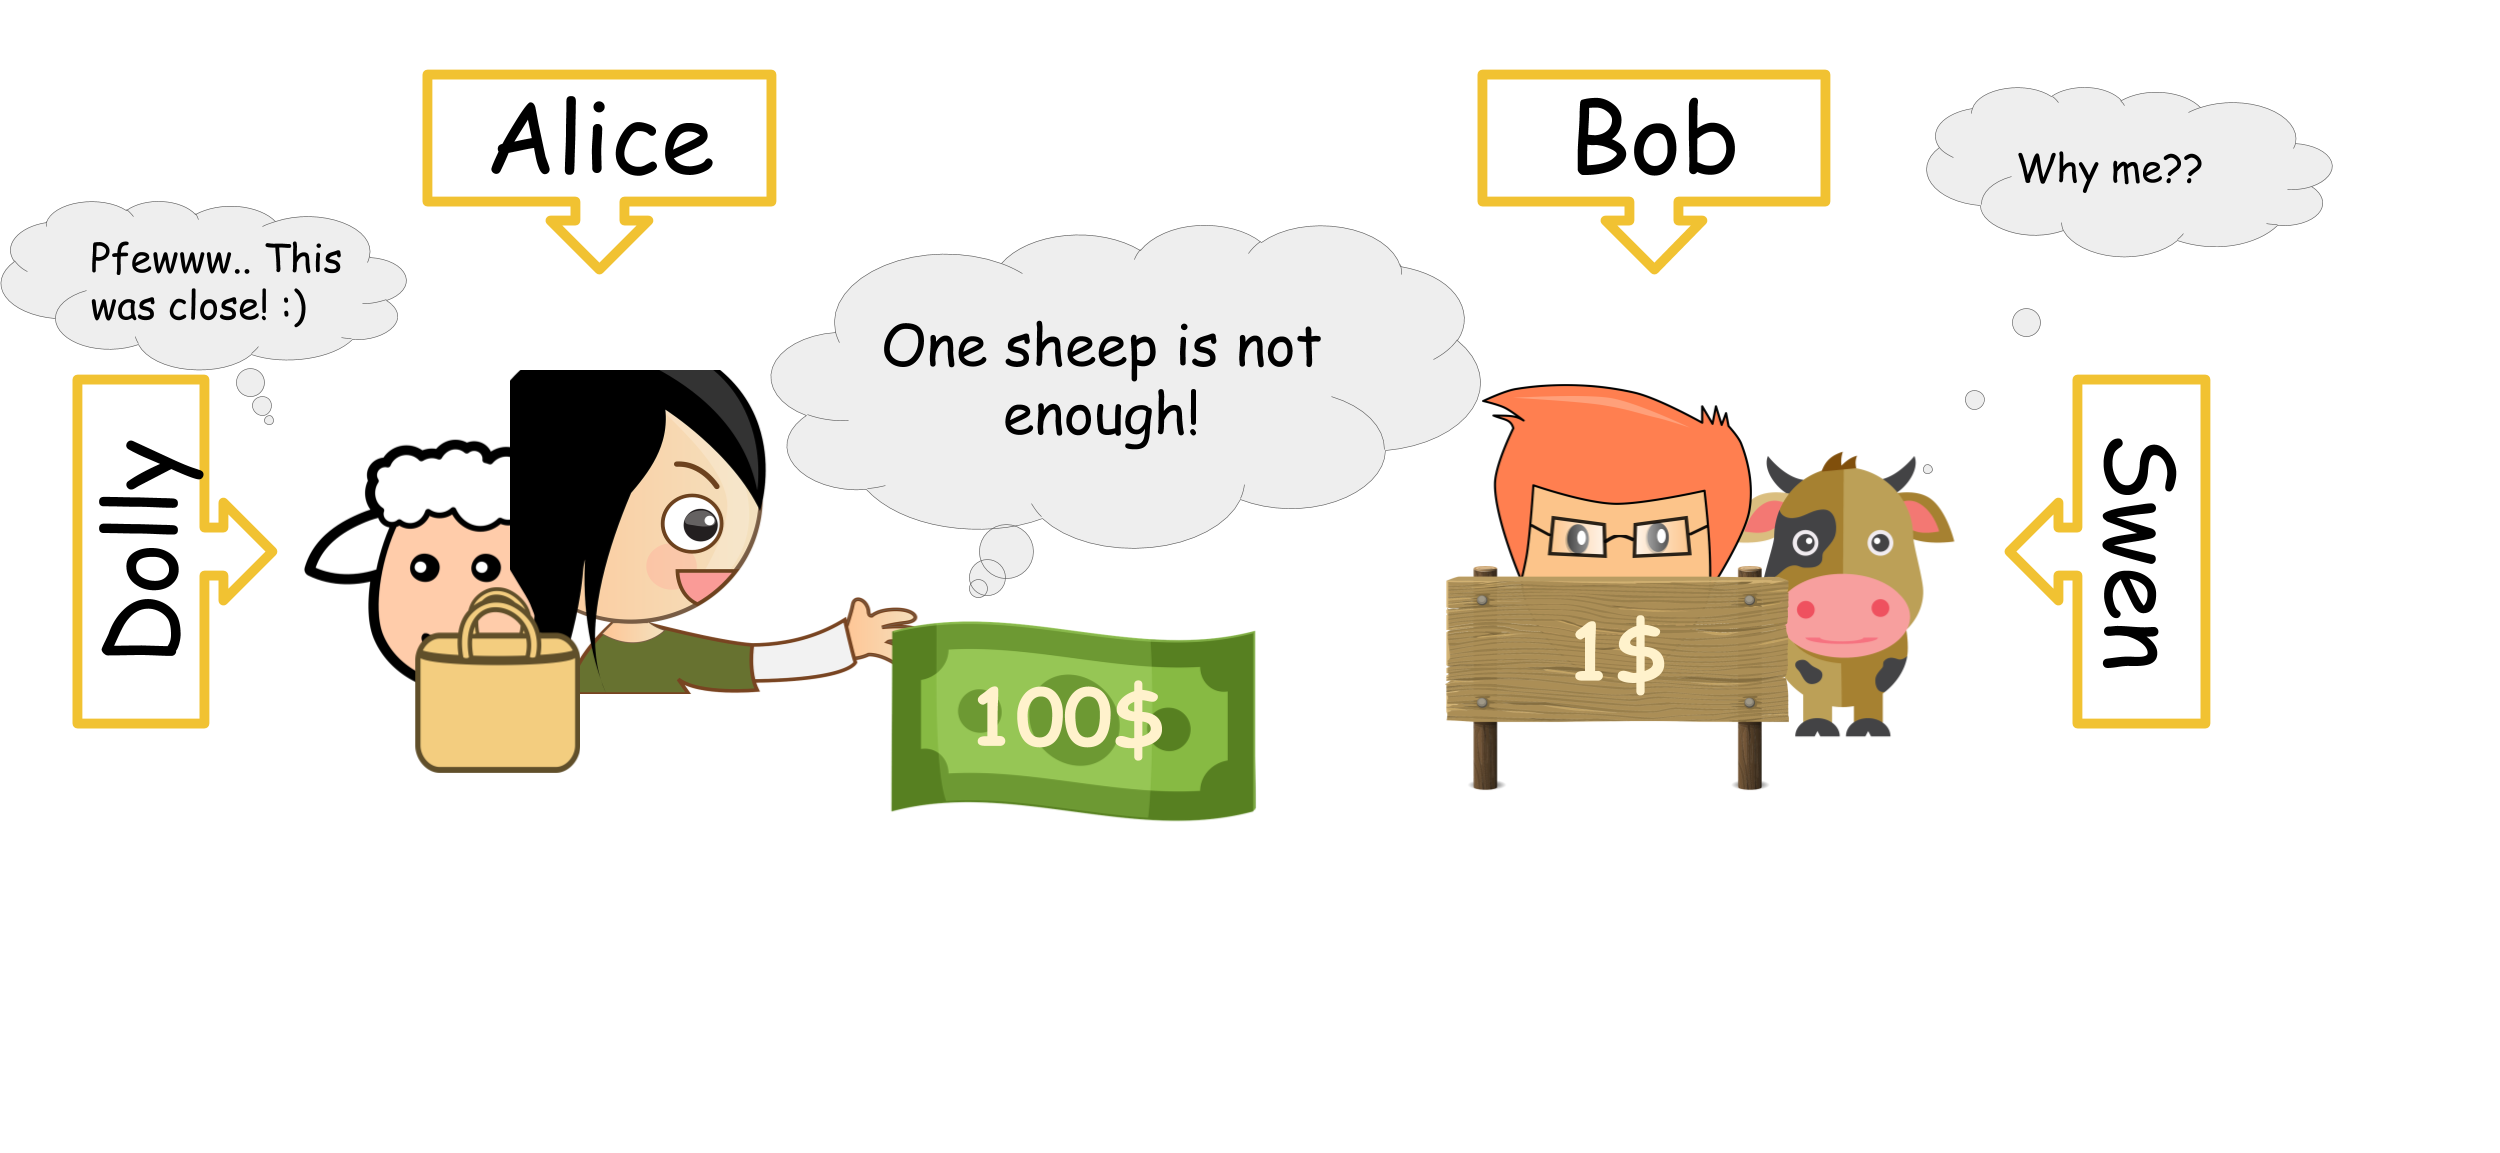
\includegraphics[width=\linewidth]{./pics/used/sheep_example_wba_mca.png}
	\end{figure}
\end{frame}

\begin{frame}{Measuring money in effective circulation---whole bill approach}
	\begin{figure}[h]
		\centering
		\inputTikz{mcirc_conceptWBA}
	\end{figure}
\end{frame}
%
\begin{frame}{Measuring money in effective circulation---moved coins approach}
	\begin{figure}[h]
		\centering
		\inputTikz{mcirc_conceptMCA}
	\end{figure}
\end{frame}
%
%==============================================================================%

% \begin{frame}{Approximations}

%   \begin{itemize}
%   \item Coin Days Destroyed (Bitcointalk.org, 2011)
%   \item Coin-Turnover (Smith, 2017)
%   \end{itemize}

% \end{frame}
